\documentclass[aspectratio=169,11pt]{beamer}
\usepackage[utf8]{inputenc}
\usepackage[T1]{fontenc}
\usepackage[scaled=1.02]{helvet}
\renewcommand{\familydefault}{\sfdefault}
\usepackage{tikz}
\usepackage{array}
\usetikzlibrary{arrows.meta,positioning,calc,fit,shapes.misc}

% ---- the game palette ----
\definecolor{gmbg}{HTML}{0B0710}     % background
\definecolor{gmpanel}{HTML}{1C1119}  % panel
\definecolor{coral}{HTML}{E08D6D}    % accent coral
\definecolor{cream}{HTML}{F2E8DC}    % text cream
\definecolor{gold}{HTML}{FFD87A}     % gold
\definecolor{teal}{HTML}{7FE9D6}     % teal

\setbeamercolor{background canvas}{bg=gmbg}
\setbeamercolor{normal text}{fg=cream}
\setbeamercolor{structure}{fg=coral}
\setbeamercolor{frametitle}{fg=cream,bg=gmbg}
\setbeamercolor{title}{fg=cream}
\setbeamercolor{itemize/enumerate body}{fg=cream}
\setbeamercolor{itemize/enumerate subbody}{fg=cream}
\setbeamerfont{frametitle}{size=\LARGE,series=\bfseries}
\setbeamerfont{title}{size=\Huge,series=\bfseries}
\setbeamertemplate{navigation symbols}{}
\setbeamertemplate{itemize item}{\textcolor{coral}{\rule[0.42ex]{0.72ex}{0.72ex}}}
\setbeamertemplate{itemize subitem}{\textcolor{gold}{--}}
\setbeamertemplate{frametitle}{%
  \vspace*{0.8em}\usebeamerfont{frametitle}\insertframetitle\par
  \vspace{0.28em}{\color{coral}\hrule height 1.4pt}\vspace{0.35em}}
\setbeamertemplate{footline}{\hfill{\color{cream!45!gmbg}\scriptsize\insertframenumber\hspace{2em}}\vspace{0.6em}}
\setbeamersize{text margin left=1.0cm,text margin right=1.0cm}

\newcommand{\kicker}[1]{{\color{coral}\scriptsize\bfseries\MakeUppercase{#1}}\\[0.3em]}
\newcommand{\dimt}[1]{{\color{cream!62!gmbg}#1}}
\newcommand{\goldb}[1]{{\color{gold}\textbf{#1}}}
\newcommand{\tealb}[1]{{\color{teal}\textbf{#1}}}

% shared tikz styles
\tikzset{
  panelbox/.style={draw=cream!22!gmbg, fill=gmpanel, rounded corners=3pt,
                   inner sep=7pt, align=center, text=cream, font=\small},
  gembox/.style={draw=coral, line width=1.3pt, fill=gmpanel, rounded corners=3pt,
                 inner sep=7pt, align=center, text=cream, font=\small},
  codebox/.style={draw=teal, line width=1.3pt, fill=gmpanel, rounded corners=3pt,
                  inner sep=7pt, align=center, text=cream, font=\small},
  goldbox/.style={draw=gold, line width=1.3pt, fill=gmpanel, rounded corners=3pt,
                  inner sep=7pt, align=center, text=cream, font=\small},
  arr/.style={-{Stealth[length=2.8mm]}, line width=1.2pt, color=coral},
  tarr/.style={-{Stealth[length=2.8mm]}, line width=1.2pt, color=teal},
  garr/.style={-{Stealth[length=2.8mm]}, line width=1.2pt, color=gold}}

\title{Gemma Monsters}
\author{}
\date{}

\begin{document}

% ================================================================ 1 · TITLE
\begin{frame}
  \begin{center}
    \vspace{1.1em}
    \kicker{Kaggle · Build with AI --- Gemma Hackathon · GDG Windsor · Edge / On-Device track}
    {\fontsize{40}{44}\selectfont\bfseries\color{cream} GEMMA \textcolor{coral}{MONSTERS}\par}
    \vspace{0.55em}
    {\Large A monster-battling castle with a real tutoring agent inside.\par}
    \vspace{0.55em}
    {\color{gold}\large Five monsters guard the Citadel. Each one is a trick --- a wrong idea that feels right.\par}
    \vspace{0.35em}
    \dimt{Powered by Gemma, running entirely on one laptop. Nothing a student does ever leaves it.}\par
    \vspace{1.5em}
    {\small Gokulakrishnan \,\textcolor{coral}{·}\, Padmanabha \,\textcolor{coral}{·}\, Taha \,\textcolor{coral}{·}\, Naimah \,\textcolor{coral}{·}\, Amarah}
  \end{center}
\end{frame}

% ================================================================ 2 · PROBLEM
\begin{frame}{Wrong answers are not random}
  \begin{center}
    \vspace{0.3em}
    {\fontsize{34}{40}\selectfont
      $\dfrac{2}{3}+\dfrac{1}{4}\;=\;$\textcolor{coral}{$\dfrac{3}{7}$}\par}
    \vspace{0.5em}
    {\large Tops with tops, bottoms with bottoms. Feels tidy. Completely wrong.\par}
    \vspace{0.9em}
    {\color{gold}\Large\bfseries That is a trick: the wrong idea that feels right.\par}
    \vspace{0.9em}
    \begin{minipage}{0.86\textwidth}\centering
      \dimt{\large This student does not need more practice --- they need that one idea found and removed.
      Practice apps mark the answer wrong and move on. Cloud tutors need the internet, ship a child's
      work to a server, and sometimes invent mathematics.}
    \end{minipage}
  \end{center}
\end{frame}

% ================================================================ 3 · MONSTERS
\begin{frame}{So we turned every trick into a monster}
  A gothic castle built in three.js. Five monsters on floating platforms, each one \emph{being} a trick.\par
  \vspace{0.15em}
  \renewcommand{\arraystretch}{1.35}
  {\footnotesize
  \begin{tabular}{@{}p{2.0cm}p{4.1cm}>{\raggedright\arraybackslash}p{6.9cm}@{}}
    {\color{gold}\bfseries Monster} & {\color{gold}\bfseries Guards the strand} & {\color{gold}\bfseries The trick it plants in your head} \\
    \multicolumn{3}{@{}c@{}}{{\color{coral}\rule[0.6ex]{13.0cm}{1.2pt}}} \\
    \textbf{Fractis}    & Number & ``just add fractions straight across'' \\
    \textbf{Equazor}    & Algebra & signs that flip when crossing the equals sign \\
    \textbf{Statiq}     & Data & mean and median blurred into one fuzzy word \\
    \textbf{Polygor}    & Geometry \& Measurement & stolen formulas that \emph{almost} fit \\
    \textbf{Ledgerling} & Financial Literacy & interest quietly skimmed off a sloppy budget \\
  \end{tabular}}
  \vspace{0.35em}

  {\color{gold}\small You beat a monster by proving its trick no longer fools you --- never by luck.}\par
  \vspace{0.1em}
  \dimt{\small Beat all five and the golden gate opens: someone is locked in the keep --- the rescue finale.}
\end{frame}

% ================================================================ 4 · EQAO
\begin{frame}{Built on the real Grade 9 curriculum}
  {\large Ontario \goldb{MTH1W} --- the course behind the Grade 9 EQAO assessment. All five strands, one monster each.\par}
  \vspace{0.4em}
  \begin{center}
  \resizebox{0.94\textwidth}{!}{%
  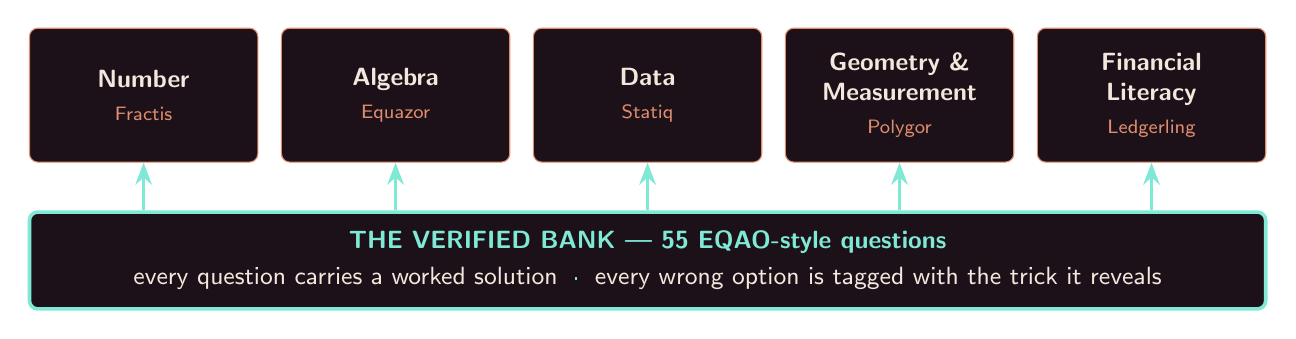
\begin{tikzpicture}[strand/.style={panelbox, minimum width=2.9cm, minimum height=1.7cm, font=\small}]
    \node[strand, draw=coral] (s1) at (0,0)    {\textbf{Number}\\[1pt]\scriptsize\color{coral} Fractis};
    \node[strand, draw=coral] (s2) at (3.2,0)  {\textbf{Algebra}\\[1pt]\scriptsize\color{coral} Equazor};
    \node[strand, draw=coral] (s3) at (6.4,0)  {\textbf{Data}\\[1pt]\scriptsize\color{coral} Statiq};
    \node[strand, draw=coral] (s4) at (9.6,0)  {\textbf{Geometry \&}\\ \textbf{Measurement}\\[1pt]\scriptsize\color{coral} Polygor};
    \node[strand, draw=coral] (s5) at (12.8,0) {\textbf{Financial}\\ \textbf{Literacy}\\[1pt]\scriptsize\color{coral} Ledgerling};
    \node[codebox, minimum width=15.7cm, font=\small] (bank) at (6.4,-2.1)
      {\tealb{THE VERIFIED BANK --- 55 EQAO-style questions}\\[2pt]
       every question carries a worked solution \;\textcolor{teal}{·}\;
       every wrong option is tagged with the trick it reveals};
    \draw[tarr] (bank.north -| s1) -- (s1.south);
    \draw[tarr] (bank.north -| s2) -- (s2.south);
    \draw[tarr] (bank.north -| s3) -- (s3.south);
    \draw[tarr] (bank.north -| s4) -- (s4.south);
    \draw[tarr] (bank.north -| s5) -- (s5.south);
  \end{tikzpicture}}
  \end{center}
  \vspace{0.45em}
  {\large So when a student picks a wrong answer, \goldb{the wrong answer itself is the diagnosis} --- a table lookup, not a model guess.\par}
  \vspace{0.45em}
  {\small Every item maps to a published MTH1W expectation and \goldb{sits inside what the EQAO
  assessment covers} --- in Financial Literacy, students \tealb{compare} the effects of rates
  and payment terms.}
\end{frame}

% ================================================================ 5 · JOURNEY
\begin{frame}{One session, start to finish}
  \begin{center}
  \resizebox{0.98\textwidth}{!}{%
  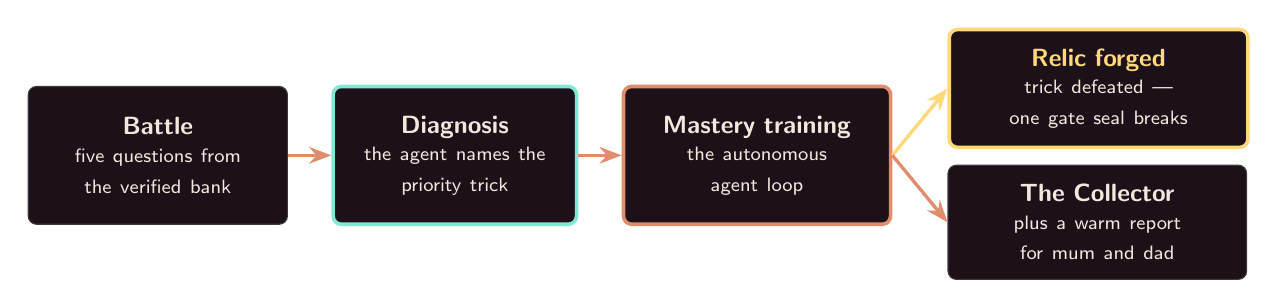
\begin{tikzpicture}[node distance=0.5cm and 0.55cm]
    \node[panelbox, minimum height=1.75cm, text width=2.8cm] (fight)
      {\textbf{Battle}\\[2pt]\scriptsize five questions from\\ \scriptsize the verified bank};
    \node[codebox, minimum height=1.75cm, text width=2.6cm, right=of fight] (diag)
      {\textbf{Diagnosis}\\[2pt]\scriptsize the agent names the\\ \scriptsize priority trick};
    \node[gembox, minimum height=1.75cm, text width=2.9cm, right=of diag] (loop)
      {\textbf{Mastery training}\\[2pt]\scriptsize the autonomous\\ \scriptsize agent loop};
    \node[goldbox, text width=3.3cm, above right=0.85cm and 0.7cm of loop.east, anchor=west] (relic)
      {\textbf{\textcolor{gold}{Relic forged}}\\[2pt]\scriptsize trick defeated ---\\ \scriptsize one gate seal breaks};
    \node[panelbox, text width=3.3cm, below right=0.85cm and 0.7cm of loop.east, anchor=west] (coll)
      {\textbf{The Collector}\\[2pt]\scriptsize plus a warm report\\ \scriptsize for mum and dad};
    \draw[arr] (fight) -- (diag);
    \draw[arr] (diag) -- (loop);
    \draw[garr] (loop.east) -- (relic.west);
    \draw[arr] (loop.east) -- (coll.west);
  \end{tikzpicture}}
  \end{center}
  \vspace{0.55em}
  \begin{itemize}\setlength\itemsep{0.4em}
    \item The monster meets you \textbf{by name} --- and it \goldb{remembers}: Gemma writes its greeting from your real battle history.
    \item Between battles: \textbf{90-second mental-math skirmishes} against the Collector's lieutenants, and his three-life \textbf{boss speed trial}.
    \item Defeat all five monsters \,$\rightarrow$\, the golden gate opens \,$\rightarrow$\, \goldb{the rescue finale}.
  \end{itemize}
\end{frame}

% ================================================================ 6 · AGENT LOOP (TikZ 1)
\begin{frame}{The agent loop: teach until the trick is gone}
  \begin{columns}[T]
    \begin{column}{0.62\textwidth}
      \begin{center}
      \resizebox{\columnwidth}{!}{%
      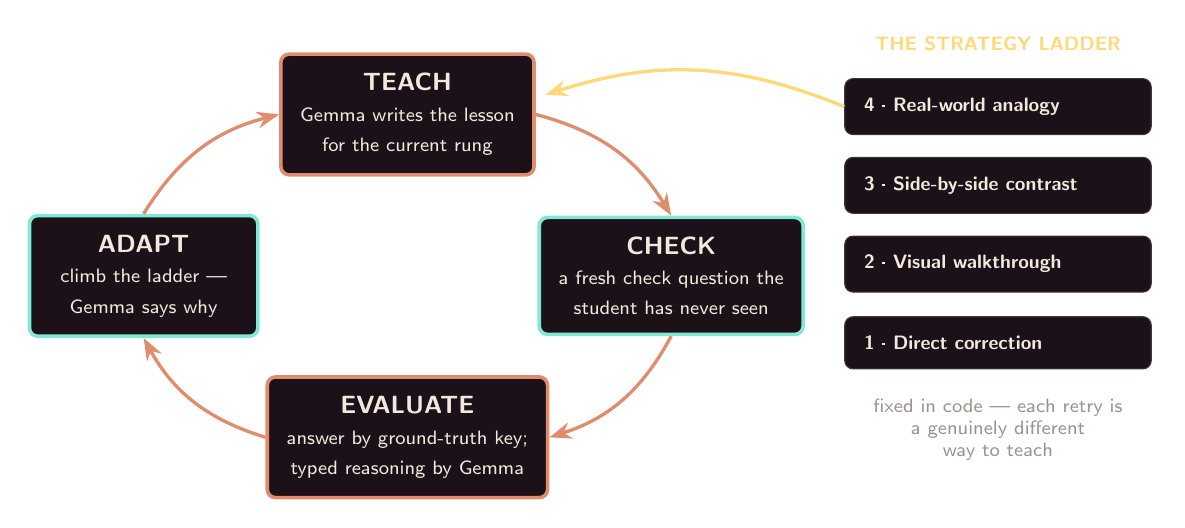
\begin{tikzpicture}
        \node[gembox, minimum width=2.9cm]  (teach) at (0,2.05)
          {\textbf{TEACH}\\ \scriptsize Gemma writes the lesson\\ \scriptsize for the current rung};
        \node[codebox, minimum width=2.9cm] (check) at (3.35,0)
          {\textbf{CHECK}\\ \scriptsize a fresh check question the\\ \scriptsize student has never seen};
        \node[gembox, minimum width=2.9cm]  (eval) at (0,-2.05)
          {\textbf{EVALUATE}\\ \scriptsize answer by ground-truth key;\\ \scriptsize typed reasoning by Gemma};
        \node[codebox, minimum width=2.9cm] (adapt) at (-3.35,0)
          {\textbf{ADAPT}\\ \scriptsize climb the ladder ---\\ \scriptsize Gemma says why};
        \draw[arr] (teach.east) to[bend left=22] (check.north);
        \draw[arr] (check.south) to[bend left=22] (eval.east);
        \draw[arr] (eval.west) to[bend left=22] (adapt.south);
        \draw[arr] (adapt.north) to[bend left=22] (teach.west);
        % the strategy ladder
        \node[panelbox, align=left, text width=3.4cm, font=\scriptsize] (l4) at (7.5,2.15)
          {\textbf{4 · Real-world analogy}};
        \node[panelbox, align=left, text width=3.4cm, font=\scriptsize] (l3) at (7.5,1.15)
          {\textbf{3 · Side-by-side contrast}};
        \node[panelbox, align=left, text width=3.4cm, font=\scriptsize] (l2) at (7.5,0.15)
          {\textbf{2 · Visual walkthrough}};
        \node[panelbox, align=left, text width=3.4cm, font=\scriptsize] (l1) at (7.5,-0.85)
          {\textbf{1 · Direct correction}};
        \node[font=\scriptsize\bfseries, text=gold] at (7.5,2.95) {THE STRATEGY LADDER};
        \node[font=\scriptsize, text=cream!62!gmbg, align=center, text width=3.8cm] at (7.5,-1.95)
          {fixed in code --- each retry is\\ a genuinely different\\ way to teach};
        \draw[garr] (l4.west) to[bend right=20] ($(teach.east)+(0.12,0.25)$);
      \end{tikzpicture}}
      \end{center}
    \end{column}
    \begin{column}{0.36\textwidth}
      \vspace{0.3em}
      {\footnotesize \tealb{Teal = code decides.} \textcolor{coral}{\textbf{Coral = Gemma judges.}}\par
      \vspace{0.55em}
      \textbf{Deterministic spine:} plain code runs the loop; Gemma is called only at the judgment points.\par
      \vspace{0.55em}
      \textbf{Two exits, no third:} two fresh correct answers with solid reasoning \goldb{forges a relic}; a spent ladder means a \textbf{warm report for mum and dad}. The agent never gives up silently.\par
      \vspace{0.55em}
      \dimt{Every switch of strategy is announced on screen, with its reason.}\par}
    \end{column}
  \end{columns}
\end{frame}

% ================================================================ 7 · REASONING GATE
\begin{frame}{A right answer is not enough}
  After every check question, the student must \goldb{type why} --- and Gemma grades those words.\par
  \vspace{0.35em}
  \begin{columns}[T]
    \begin{column}{0.5\textwidth}
      \begin{center}
      \begin{tikzpicture}
        \node[panelbox, align=left, text width=6.0cm, font=\footnotesize] {
          {\scriptsize\color{cream!62!gmbg} THE CHECK QUESTION}\\[1pt]
          Calculate $\tfrac{1}{2}+\tfrac{1}{3}$ \;---\; picks \textbf{$\tfrac{5}{6}$}\, \textcolor{teal}{(correct)}\\[5pt]
          {\scriptsize\color{cream!62!gmbg} THE STUDENT TYPES}\\[1pt]
          \emph{``I just guessed the biggest fraction''}\\[5pt]
          {\scriptsize\color{cream!62!gmbg} GEMMA'S GRADE}\\[1pt]
          {\color{coral}\textbf{SHALLOW}} --- does \textbf{not} count toward mastery};
      \end{tikzpicture}
      \end{center}
    \end{column}
    \begin{column}{0.47\textwidth}
      {\footnotesize
      \begin{itemize}\setlength\itemsep{0.5em}
        \item Three labels only --- \textbf{RESOLVED / SHALLOW / SAME\_ERROR}. A closed set, nothing open-ended.
        \item The monster \goldb{answers the student's own words back, in character} --- it read what you wrote.
        \item \tealb{Fail-open:} if the grader hiccups, the student is never punished for it.
      \end{itemize}}
    \end{column}
  \end{columns}
  \vspace{0.25em}
  {\color{gold} A lucky bubble cannot fake understanding past this gate.}
\end{frame}

% ================================================================ 8 · ARCHITECTURE (TikZ 2)
\begin{frame}{Everything on one laptop}
  \begin{center}
  \resizebox{0.78\textwidth}{!}{%
  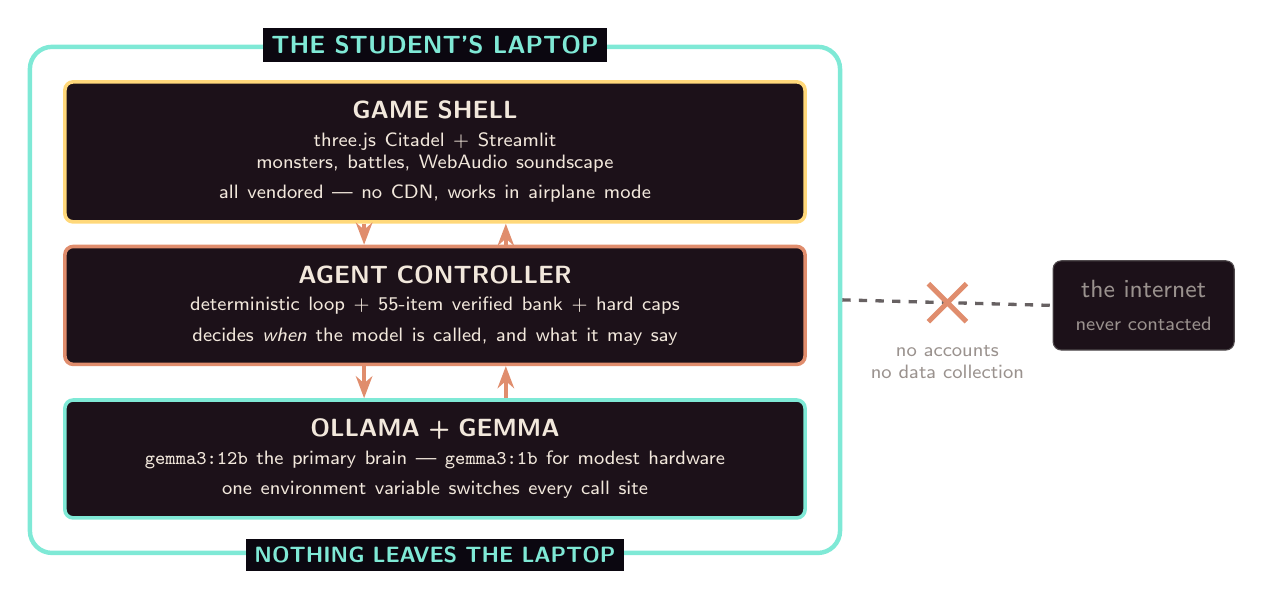
\begin{tikzpicture}
    \node[goldbox, minimum width=9.4cm, text width=8.8cm] (game) at (0,2.5)
      {\textbf{GAME SHELL}\\[2pt]\scriptsize three.js Citadel + Streamlit\\
       \scriptsize monsters, battles, WebAudio soundscape\\
       \scriptsize all vendored --- no CDN, works in airplane mode};
    \node[gembox, minimum width=9.4cm, text width=8.8cm] (agent) at (0,0.55)
      {\textbf{AGENT CONTROLLER}\\[2pt]\scriptsize deterministic loop + 55-item verified bank + hard caps\\
       \scriptsize decides \emph{when} the model is called, and what it may say};
    \node[codebox, minimum width=9.4cm, text width=8.8cm] (gemma) at (0,-1.4)
      {\textbf{OLLAMA + GEMMA}\\[2pt]\scriptsize \texttt{gemma3:12b} the primary brain --- \texttt{gemma3:1b} for modest hardware\\
       \scriptsize one environment variable switches every call site};
    \draw[arr] ($(game.south)+(-0.9,0)$) -- ($(agent.north)+(-0.9,0)$);
    \draw[arr] ($(agent.north)+(0.9,0)$) -- ($(game.south)+(0.9,0)$);
    \draw[arr] ($(agent.south)+(-0.9,0)$) -- ($(gemma.north)+(-0.9,0)$);
    \draw[arr] ($(gemma.north)+(0.9,0)$) -- ($(agent.south)+(0.9,0)$);
    % the boundary
    \node[draw=teal, line width=1.6pt, rounded corners=8pt, inner sep=12pt,
          fit=(game)(gemma)] (laptop) {};
    \node[font=\small\bfseries, text=teal, fill=gmbg, inner sep=3pt]
      at (laptop.north) {THE STUDENT'S LAPTOP};
    \node[font=\footnotesize\bfseries, text=teal, fill=gmbg, inner sep=3pt]
      at (laptop.south) {NOTHING LEAVES THE LAPTOP};
    % the internet, unreachable
    \node[panelbox, draw=cream!30!gmbg, minimum width=2.3cm, text=cream!62!gmbg] (net) at (9.0,0.55)
      {the internet\\[1pt]\scriptsize never contacted};
    \draw[line width=1.2pt, color=cream!40!gmbg, dashed] (laptop.east) -- (net.west);
    \node[cross out, draw=coral, line width=1.8pt, minimum size=0.42cm]
      at ($(laptop.east)!0.5!(net.west)$) {};
    \node[font=\scriptsize, text=cream!62!gmbg, align=center] at ($(laptop.east)!0.5!(net.west)+(0,-0.75)$)
      {no accounts\\ no data collection};
  \end{tikzpicture}}
  \end{center}
  \vspace{0.05em}
  The Edge / On-Device promise, kept literally: \goldb{a student's struggles stay on their own machine.}
\end{frame}

% ================================================================ 9 · TRUST SPLIT (TikZ 3)
\begin{frame}{Gemma judges. Code guarantees.}
  \begin{center}
  \resizebox{0.86\textwidth}{!}{%
  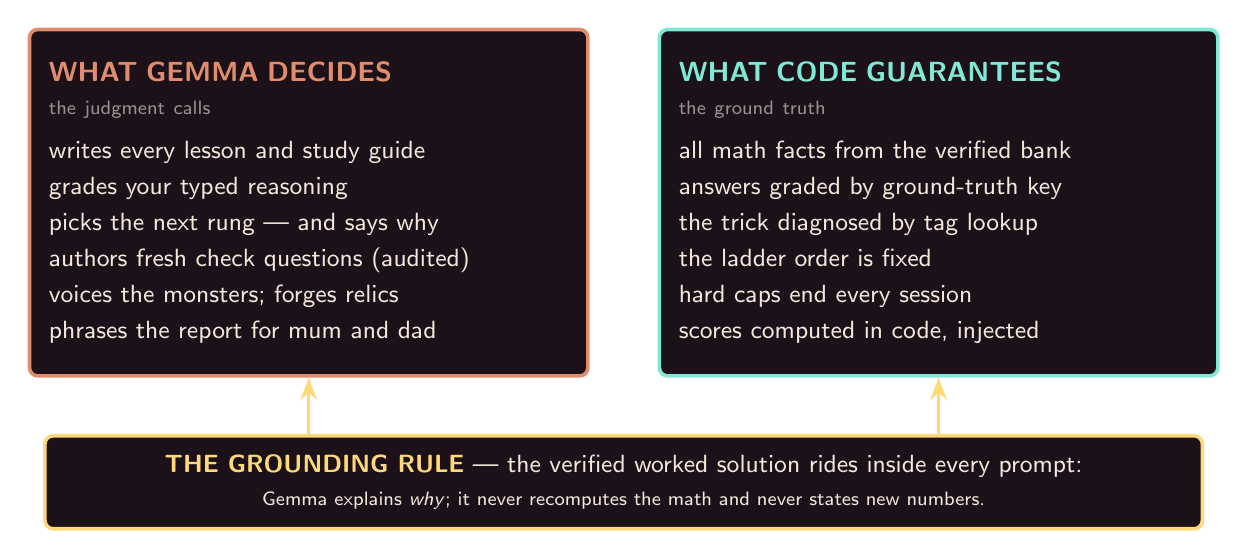
\begin{tikzpicture}
    \node[gembox, align=left, text width=6.6cm, minimum height=4.4cm, font=\small] (gem) at (0,0) {
      {\normalsize\textbf{\textcolor{coral}{WHAT GEMMA DECIDES}}}\\[1pt]
      {\scriptsize\color{cream!62!gmbg} the judgment calls}\\[5pt]
      writes every lesson and study guide\\[2pt]
      grades your typed reasoning\\[2pt]
      picks the next rung --- and says why\\[2pt]
      authors fresh check questions (audited)\\[2pt]
      voices the monsters; forges relics\\[2pt]
      phrases the report for mum and dad};
    \node[codebox, align=left, text width=6.6cm, minimum height=4.4cm, font=\small] (cod) at (8.0,0) {
      {\normalsize\textbf{\textcolor{teal}{WHAT CODE GUARANTEES}}}\\[1pt]
      {\scriptsize\color{cream!62!gmbg} the ground truth}\\[5pt]
      all math facts from the verified bank\\[2pt]
      answers graded by ground-truth key\\[2pt]
      the trick diagnosed by tag lookup\\[2pt]
      the ladder order is fixed\\[2pt]
      hard caps end every session\\[2pt]
      scores computed in code, injected};
    \node[goldbox, minimum width=14.7cm, font=\small] (bank) at (4.0,-3.55)
      {\goldb{THE GROUNDING RULE} --- the verified worked solution rides inside every prompt:\\[1pt]
       \scriptsize Gemma explains \emph{why}; it never recomputes the math and never states new numbers.};
    \draw[garr] (bank.north -| gem) -- (gem.south);
    \draw[garr] (bank.north -| cod) -- (cod.south);
  \end{tikzpicture}}
  \end{center}
  \vspace{0.1em}
  The model does the thinking --- \goldb{it is never the source of mathematical truth.}
\end{frame}

% ================================================================ 10 · SAFETY NET
\begin{frame}{We planned for the model to fail}
  Every guardrail exists because live testing broke something first.\par
  \vspace{0.25em}
  \begin{columns}[T]
    \begin{column}{0.49\textwidth}
      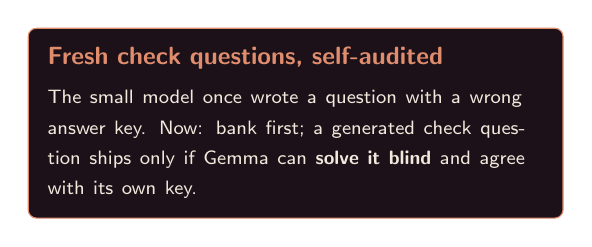
\begin{tikzpicture}
        \node[panelbox, draw=coral, align=left, text width=6.3cm, font=\small] {
          {\textbf{\textcolor{coral}{Fresh check questions, self-audited}}}\\[3pt]
          \scriptsize The small model once wrote a question with a wrong
          answer key. Now: bank first; a generated check question ships only if Gemma
          can \textbf{solve it blind} and agree with its own key.};
      \end{tikzpicture}\\[0.25em]
      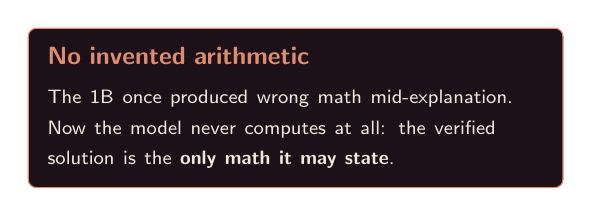
\begin{tikzpicture}
        \node[panelbox, draw=coral, align=left, text width=6.3cm, font=\small] {
          {\textbf{\textcolor{coral}{No invented arithmetic}}}\\[3pt]
          \scriptsize The 1B once produced wrong math mid-explanation. Now the model
          never computes at all: the verified solution is the \textbf{only math it may state}.};
      \end{tikzpicture}
    \end{column}
    \begin{column}{0.49\textwidth}
      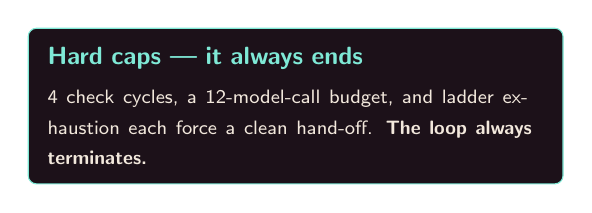
\begin{tikzpicture}
        \node[panelbox, draw=teal, align=left, text width=6.3cm, font=\small] {
          {\textbf{\textcolor{teal}{Hard caps --- it always ends}}}\\[3pt]
          \scriptsize 4 check cycles, a 12-model-call budget, and ladder exhaustion
          each force a clean hand-off. \textbf{The loop always terminates.}};
      \end{tikzpicture}\\[0.25em]
      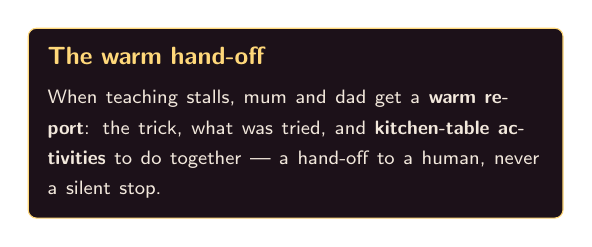
\begin{tikzpicture}
        \node[panelbox, draw=gold, align=left, text width=6.3cm, font=\small] {
          {\textbf{\textcolor{gold}{The warm hand-off}}}\\[3pt]
          \scriptsize When teaching stalls, mum and dad get a \textbf{warm report}:
          the trick, what was tried, and \textbf{kitchen-table activities} to do together
          --- a hand-off to a human, never a silent stop.};
      \end{tikzpicture}
    \end{column}
  \end{columns}
  \vspace{0.05em}
  {\color{gold}\small The guardrails carry correctness; model size only dials quality.}
\end{frame}

% ================================================================ 11 · RUBRIC
\begin{frame}{What we would want a judge to notice}
  \vspace{0.2em}
  \begin{columns}[T]
    \begin{column}{0.24\textwidth}
      {\color{coral}\small\textbf{GEMMA IS THE ENGINE}}\par
      \vspace{0.4em}{\color{coral}\hrule height 1.2pt}\vspace{0.5em}
      {\footnotesize
      Ten call sites behind one auditable door: lessons, reasoning grades,
      strategy picks, check questions, coaching, relics, reports, and the
      director that decides where the student goes next.\\[3pt]
      Fully local through Ollama --- \texttt{gemma3:12b}, with \texttt{1b} one flag away.}
    \end{column}
    \begin{column}{0.24\textwidth}
      {\color{gold}\small\textbf{NOBODY HAS BUILT THIS}}\par
      \vspace{0.4em}{\color{gold}\hrule height 1.2pt}\vspace{0.5em}
      {\footnotesize
      A tutoring agent you can \emph{fight}: every trick embodied as a monster
      that has to be beaten on understanding.\\[3pt]
      Mastery is gated on the student's own typed reasoning --- and the citadel
      answers those words back.}
    \end{column}
    \begin{column}{0.24\textwidth}
      {\color{teal}\small\textbf{IT ACTUALLY RUNS}}\par
      \vspace{0.4em}{\color{teal}\hrule height 1.2pt}\vspace{0.5em}
      {\footnotesize
      Live and end to end with the Wi-Fi off: citadel, battles, the agent loop,
      speed skirmishes, the boss trial, the rescue.\\[3pt]
      Hard caps mean no session can hang, and a model hiccup never costs the
      student anything.}
    \end{column}
    \begin{column}{0.24\textwidth}
      {\color{cream}\small\textbf{WE SHOW OUR WORK}}\par
      \vspace{0.4em}{\color{cream!45!gmbg}\hrule height 1.2pt}\vspace{0.5em}
      {\footnotesize
      An honest engineering story: what the model broke under testing, and the
      structural fix behind each guardrail.\\[3pt]
      Every item in the bank maps to a published Grade 9 expectation.}
    \end{column}
  \end{columns}
  \vspace{0.3em}
  \begin{center}
    \small\dimt{In one sentence:}\ \goldb{an autonomous, explainable, fully on-device
    tutoring agent --- wearing a monster suit.}
  \end{center}
\end{frame}

% ================================================================ 12 · CLOSE
\begin{frame}
  \begin{center}
    \vspace{1.6em}
    {\fontsize{27}{33}\selectfont\bfseries\color{cream} Every monster is a trick ---\\ a wrong idea that feels right.\par}
    \vspace{0.9em}
    {\Large\color{gold} Defeat the idea, and the gate opens.\par}
    \vspace{1.1em}
    \dimt{\large A student walks in adding fractions straight across. Twenty minutes later they have
    \emph{proven} the trick is gone --- and nothing about them ever left their laptop.}\par
    \vspace{1.5em}
    {\small\color{teal} github.com/EdTechDL/gemma-without-borders \,·\, live demo, Wi-Fi off \,·\, companion Kaggle notebook}\par
    \vspace{0.5em}
    {\small Gokulakrishnan \,\textcolor{coral}{·}\, Padmanabha \,\textcolor{coral}{·}\, Taha \,\textcolor{coral}{·}\, Naimah \,\textcolor{coral}{·}\, Amarah}
  \end{center}
\end{frame}

\end{document}
